\documentclass[12pt]{article}
\usepackage[utf8]{inputenc}

%%% I added a few packages. This next one allows you to set the margins.
\usepackage[top=.5in,bottom=1in,right=.75in,left=.75in]{geometry}
\usepackage{multicol}
%\usepackage{newspaper}
\setlength{\columnsep}{1cm}
\usepackage{blindtext}
\usepackage{varwidth}

%%% This one does boxes in a really nice way.
\usepackage{tcolorbox}
\usepackage{mdframed}
\usepackage{minibox}
\usepackage{graphicx}
\graphicspath{ {./images/} }
\usepackage{epstopdf}
  \epstopdfDeclareGraphicsRule{.pdf}{png}{.png}{convert #1 \OutputFile}
  \DeclareGraphicsExtensions{.png,.pdf}
\usepackage{hyperref}
\hypersetup{
    colorlinks=true,
    linkcolor=blue,
    filecolor=magenta,      
    urlcolor=cyan,
    pdftitle={MSCSMess},
    pdfpagemode=FullScreen,
    }
\urlstyle{same}
 \usepackage{fix-cm}
 \usepackage{soul}
 \usepackage{graphicx}
 \usepackage{multicol}


\newcommand{\ds}{\displaystyle}
\newcommand{\ZZ}{\mathbb{Z}}
\newcommand{\QQ}{\mathbb{Q}}
\newcommand{\RR}{\mathbb{R}}
\newcommand{\CC}{\mathbb{C}}
\newcommand{\FF}{\mathbb{F}}
\newcommand{\xx}{\mathbf{x}}
\newcommand{\uu}{\mathbf{u}}
\newcommand{\vv}{\mathbf{v}}

\newcommand{\bolder}{\textbf}
 
 
\title{\fontsize{60}{70}\selectfont {\bf {MSCS} 
\includegraphics[scale=.3]{images/OleLion.png} {Mess}}}
\author{Department of Mathematics, Statistics, and Computer Science \\ St.\@ Olaf College, Northfield, MN 55057 \vspace{-2ex}} 
\date{\today\, $|$ Volume 54, No.\@ 22 \line(1,0){500}}


\begin{document}

\maketitle \vspace{-1cm}
\begin{center}
Happy Friday! Don’t forget to take some breaks and check out all the exciting events happening around campus over the next few weeks. There’s a lot going on! Have an awesome weekend! :)

\end{center}

 \begin{multicols}{2}


 \begin{tcolorbox}[colback=white, colframe=black]
    \begin{center}
    \title{{\large \bolder{Math Education at St. Olaf}}}
    \end{center}
\end{tcolorbox}

At St. Olaf, you can double major in Mathematics and Education, complete a student-teaching semester, and graduate licensed to teach middle or high school math. Our Education program is serious about the vocation of teaching: our courses help you think deeply about what it means to teach the whole person, not just your content. And you'll spend real, meaningful time in classrooms throughout the program, learning the profession alongside practicing teachers.

To learn more, reach out to Prof. Ryota Matsuura (matsuura@stolaf.edu) or visit \href{https://pages.stolaf.edu/matsuura/math-ed-st-olaf/}{his website} for details.

P.S. We have a J-term course, Educ 378 Multicultural Education in Hawaii. Yes, it's an off-campus course!

\begin{tcolorbox}[colback=white, colframe=black]
    \begin{center}
    \title{{\large \bolder{NSM Honors Day Poster Session!}}}
    \end{center}
\end{tcolorbox}

Join us for this year’s NSM Honors Day Poster Session! We invite anyone who has completed research (on or off campus) to present their work. The event is open to everyone, and snacks and beverages will be served. Please see the \href{https://wp.stolaf.edu/physics/honorsdaypostersession_sci_math/} {NSM Honors Day Poster Session website} for more information and to register. 


\begin{tcolorbox}[colback=white, colframe=black]
    \begin{center}
    \title{{\large \bolder{4/20 MSCS Colloquium: Joslenne Peña}}}
    \end{center}
\end{tcolorbox}

Join us for an MSCS Department Colloquium on Monday, April 20th at 3:30pm in RNS 210! Our speaker, Dr. Joslenne Peña (she/her), Assistant Professor of Computer Science at Macalester College, will present "Community Coding Workshops for Life-Long Learners Using Libraries: An Informal Learning Approach". Her talk explores Code for Us (CFU), an NSF-funded program that uses libraries as hubs for teaching foundational programming skills to adult learners. All are welcome!


\begin{tcolorbox}[colback=white, colframe=black]
    \begin{center}
    \title{{\large \bolder{Mario Kart Tournament}}}
    \end{center}
\end{tcolorbox}

Rev your engines! The St. Olaf CS Department is hosting a Mario Kart Tournament on Monday, April 20th at 4:45pm in the CS Advanced Lab. Come for the epic prizes and bring your friends and competitive spirit. Get ready for a splendid time!


\begin{tcolorbox}[colback=white, colframe=black]
    \begin{center}
    \title{{\large \bolder{TLC Lecture: Deanna Haunsperger}}}
    \end{center}
\end{tcolorbox}

Don't miss the TLC Lecture featuring Deanna Haunsperger (she/her) on Friday, April 24th at 3:30pm in RNS 210, with a reception to follow in RNS 207. Her talk, "Halving Your Cake," tackles the age-old question of fair division: how do you split a resource equitably among more than two people? 

Haunsperger is a Professor of Mathematics at Carleton College, past President of the Mathematical Association of America, and co-founder of the Carleton Summer Mathematics Program for Women. We hope you'll stop by!

\begin{tcolorbox}[colback=white, colframe=black]
    \begin{center}
    \title{{\large \bolder{MSCS Grader Applications}}}
    \end{center}
\end{tcolorbox}

The MSCS department is now accepting Grader/TA applications for Fall 2026. If you are interested in working with us please \href{https://forms.gle/c9Rw2DAwuYA8vBtM9}{apply here}. The deadline for applying is Wednesday, April 22nd at 11:59pm. The qualifications are as follows: 

 \begin{itemize}
    \item Completed the course with an A or B.
    \item Ability to maintain confidentiality.
    \item Complete work in a timely manner.
    \item Availability to work the entire semester.
\end{itemize} 

\begin{tcolorbox}[colback=white, colframe=black]
    \begin{center}
    \title{{\large \bolder{4/27--4/28 Kleber-Gery Lectures: Marc Richards '16}}}
    \end{center}
\end{tcolorbox}

Marc Richards '16, Director of Football Research \& Development for the Kansas City Chiefs, is coming to campus for two Kleber-Gery events this week! On Monday, April 27th at 7:00pm in the Viking Theater, he will present The History and Lessons of Sports Analytics: How Teams Use Data-Driven Approaches to Make Decisions, tracing the evolution of sports analytics from box scores to advanced player tracking and discussing the roles that define modern analytics departments (welcome reception at 6:30pm). 

Then on Tuesday, April 28th at 3:30pm in RMS 210, he will give the Kleber-Gery Colloquium talk Moving Beyond Assists: An Analysis of Passing Ability in Hockey, introducing new metrics for quantifying pass risk and reward using player and puck tracking data from Stathletes' 2021 Big Data Cup. All are welcome at both events!

Contact Melissa Schori (schori1@stolaf.edu) if you have any questions!

\begin{tcolorbox}[colback=white, colframe=black]
    \begin{center}
    \title{{\large \bolder{MSCS Senior Banquet}}}
    \end{center}
\end{tcolorbox}

MSCS graduating seniors are invited to attend this year's Senior Banquet on May 7th at 5:30pm. Please RSVP using \href{https://docs.google.com/forms/d/e/1FAIpQLScgOKI8CBUjdAlBOWogwo_QmVcTVVHmFHDOw5-bzeL7vT30CQ/viewform}{this link} by Tuesday, April 28th. 

\begin{tcolorbox}[colback=white, colframe=black]
    \begin{center}
    \title{{\large \bolder{Computer Science Showcase}}}
    \end{center}
\end{tcolorbox}

Come see what your fellow Oles have been building! The Computer Science Showcase is on Monday, May 11th at 3:30pm in the Buntrock Commons Sun Ballroom. CS students will present their year-long projects, and there will be snacks, good vibes, and prizes up for grabs. Want to show off your own project? Scan the QR code on the poster or reach out to Prof. Leeson (leeson2@stolaf.edu) to sign up.

\begin{tcolorbox}[colback=white, colframe=black]
    \begin{center}
    \title{{\large \bolder{Have you done math research?
    }}}
    \end{center}
\end{tcolorbox}
Professor Dietz edits an annual volume of mathematics research papers written by students, whether the research was supervised by a St. Olaf faculty member or not. If you've done something original in an REU, DUR, IR/IS between about May 2025 and now, please email dietz@stolaf.edu. 

\begin{tcolorbox}[colback=white, colframe=black]
    \begin{center}
    \title{{\large \bolder{Problem Solving Group}}}
    \end{center}
\end{tcolorbox}
The Math Problem Solving Group meets weekly to have fun, solve math problems, eat candy, and prepare for upcoming math contests. Meetings are Thursdays from 11:30 am - 12:30 pm, in RNS 207 (the Center for Interdisciplinary Research room). Everyone is welcome, regardless of prior experience in mathematics or math contests!


\end{multicols} \vspace{3cm} 

A poem from Dr. Gandini:

\begin{center}
    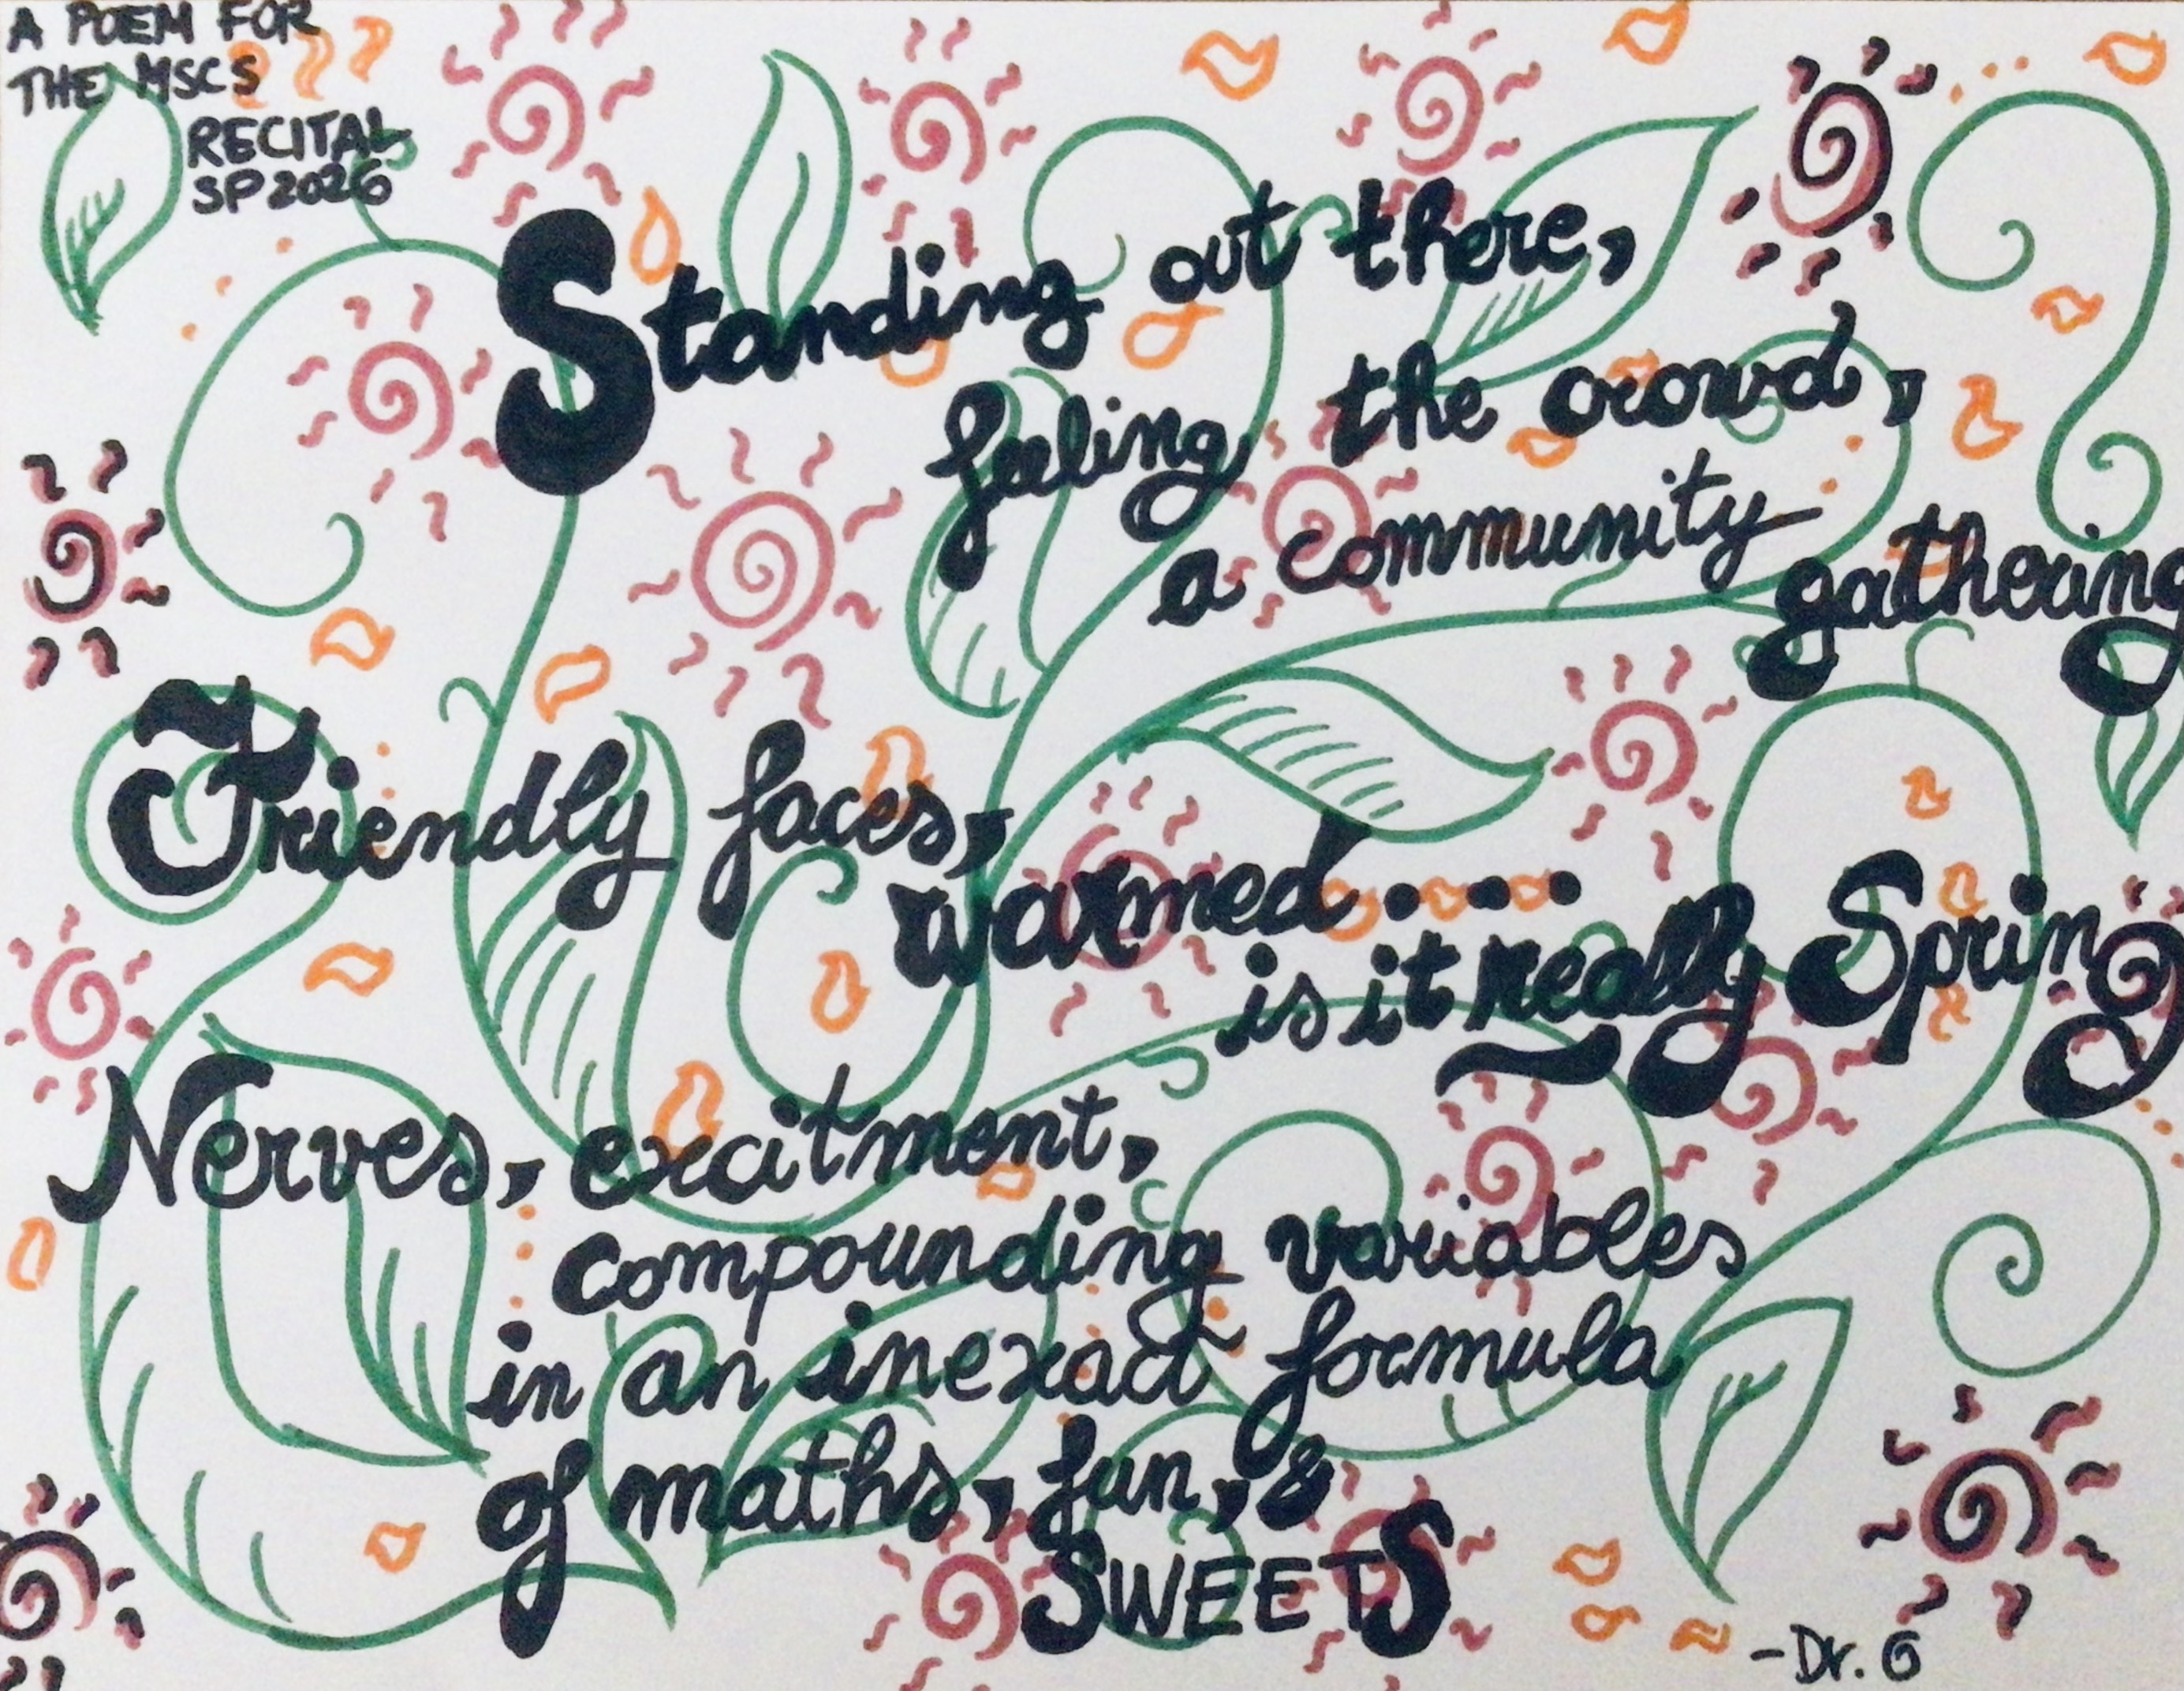
\includegraphics[width=0.9\textwidth]{images/IMG_0098.jpg}
\end{center}

\begin{center}
    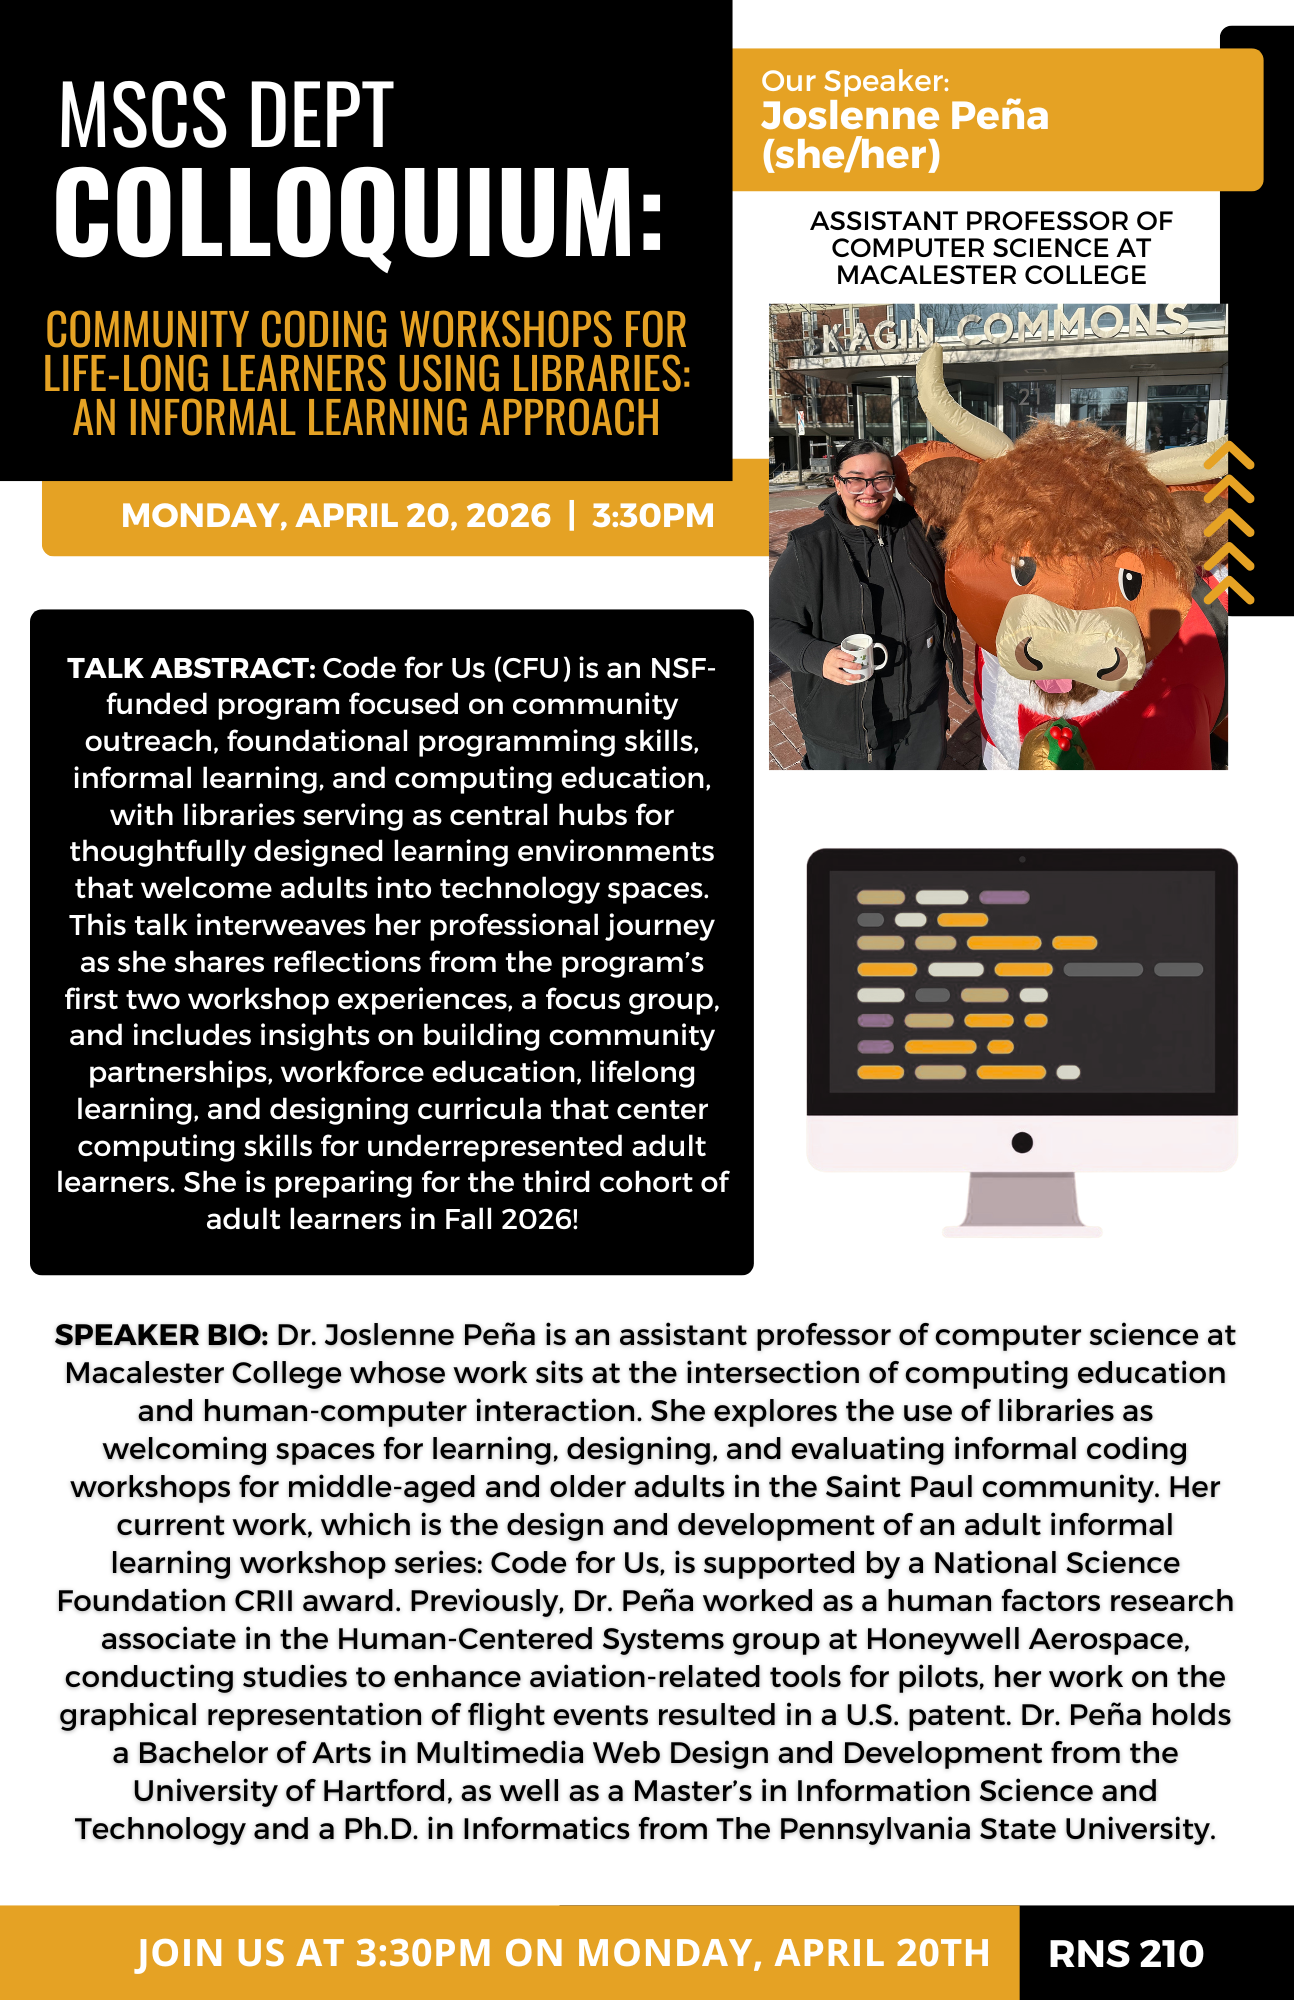
\includegraphics[height=0.95\textheight]{images/Colloquium Joslene Pena.png}
\end{center}

\begin{center}
    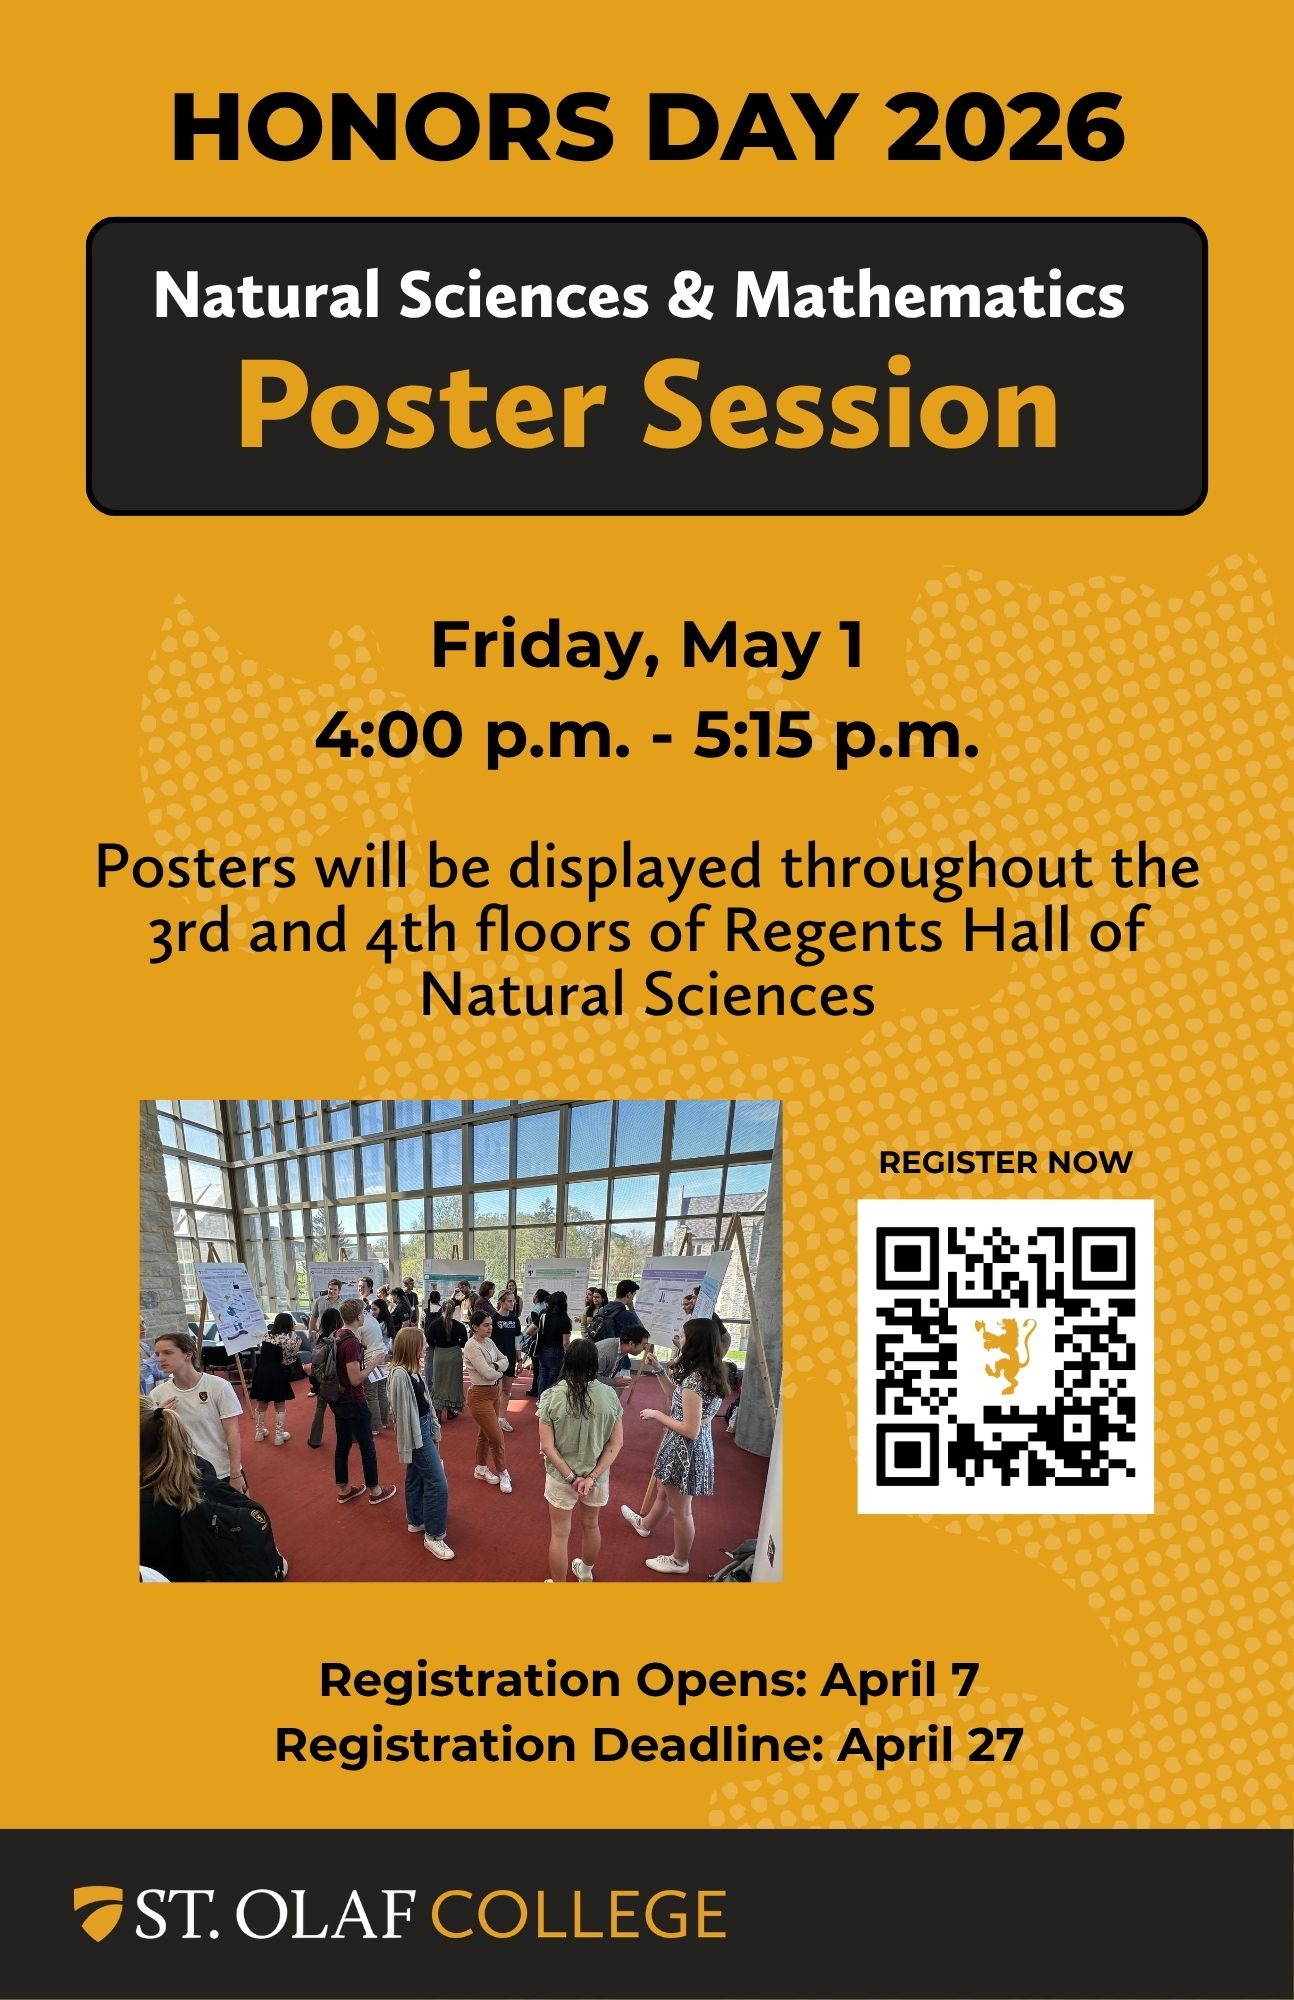
\includegraphics[height=0.95\textheight]{2026 Honors Day Poster T1 (1).jpg}
\end{center}

\begin{center}
    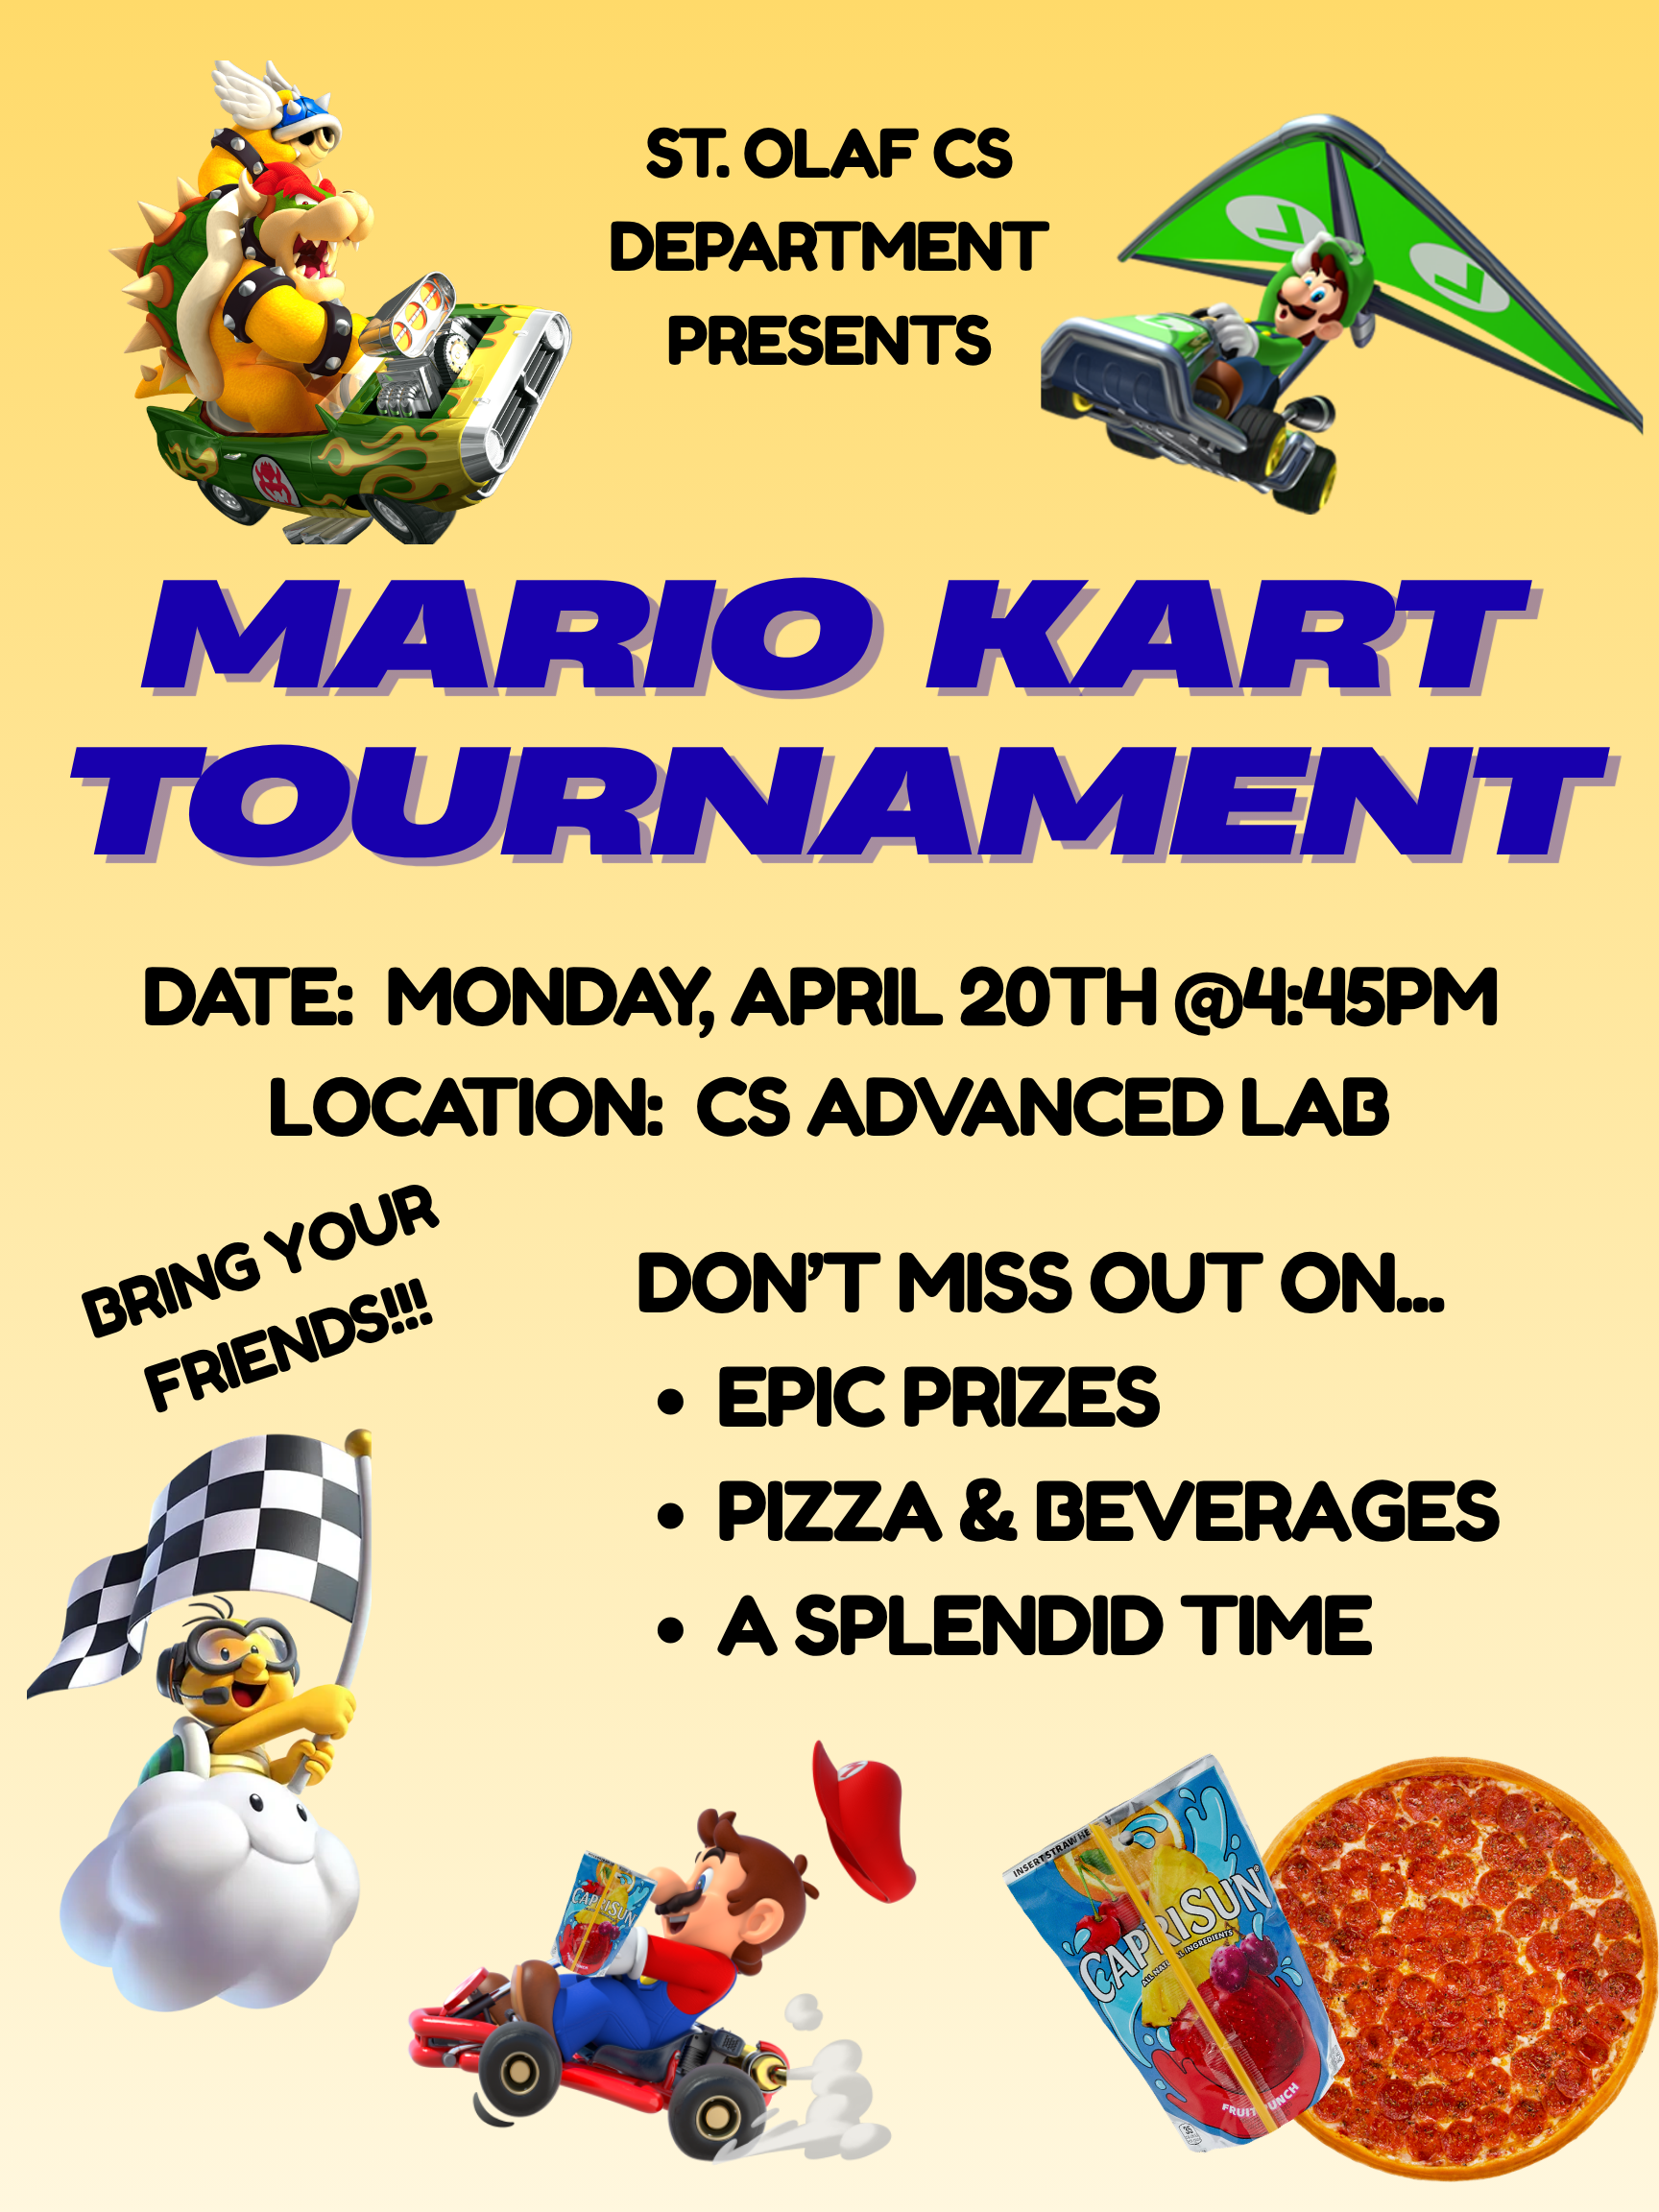
\includegraphics[height=0.95\textheight]{images/MarioKart.png}
\end{center}

\begin{center}
    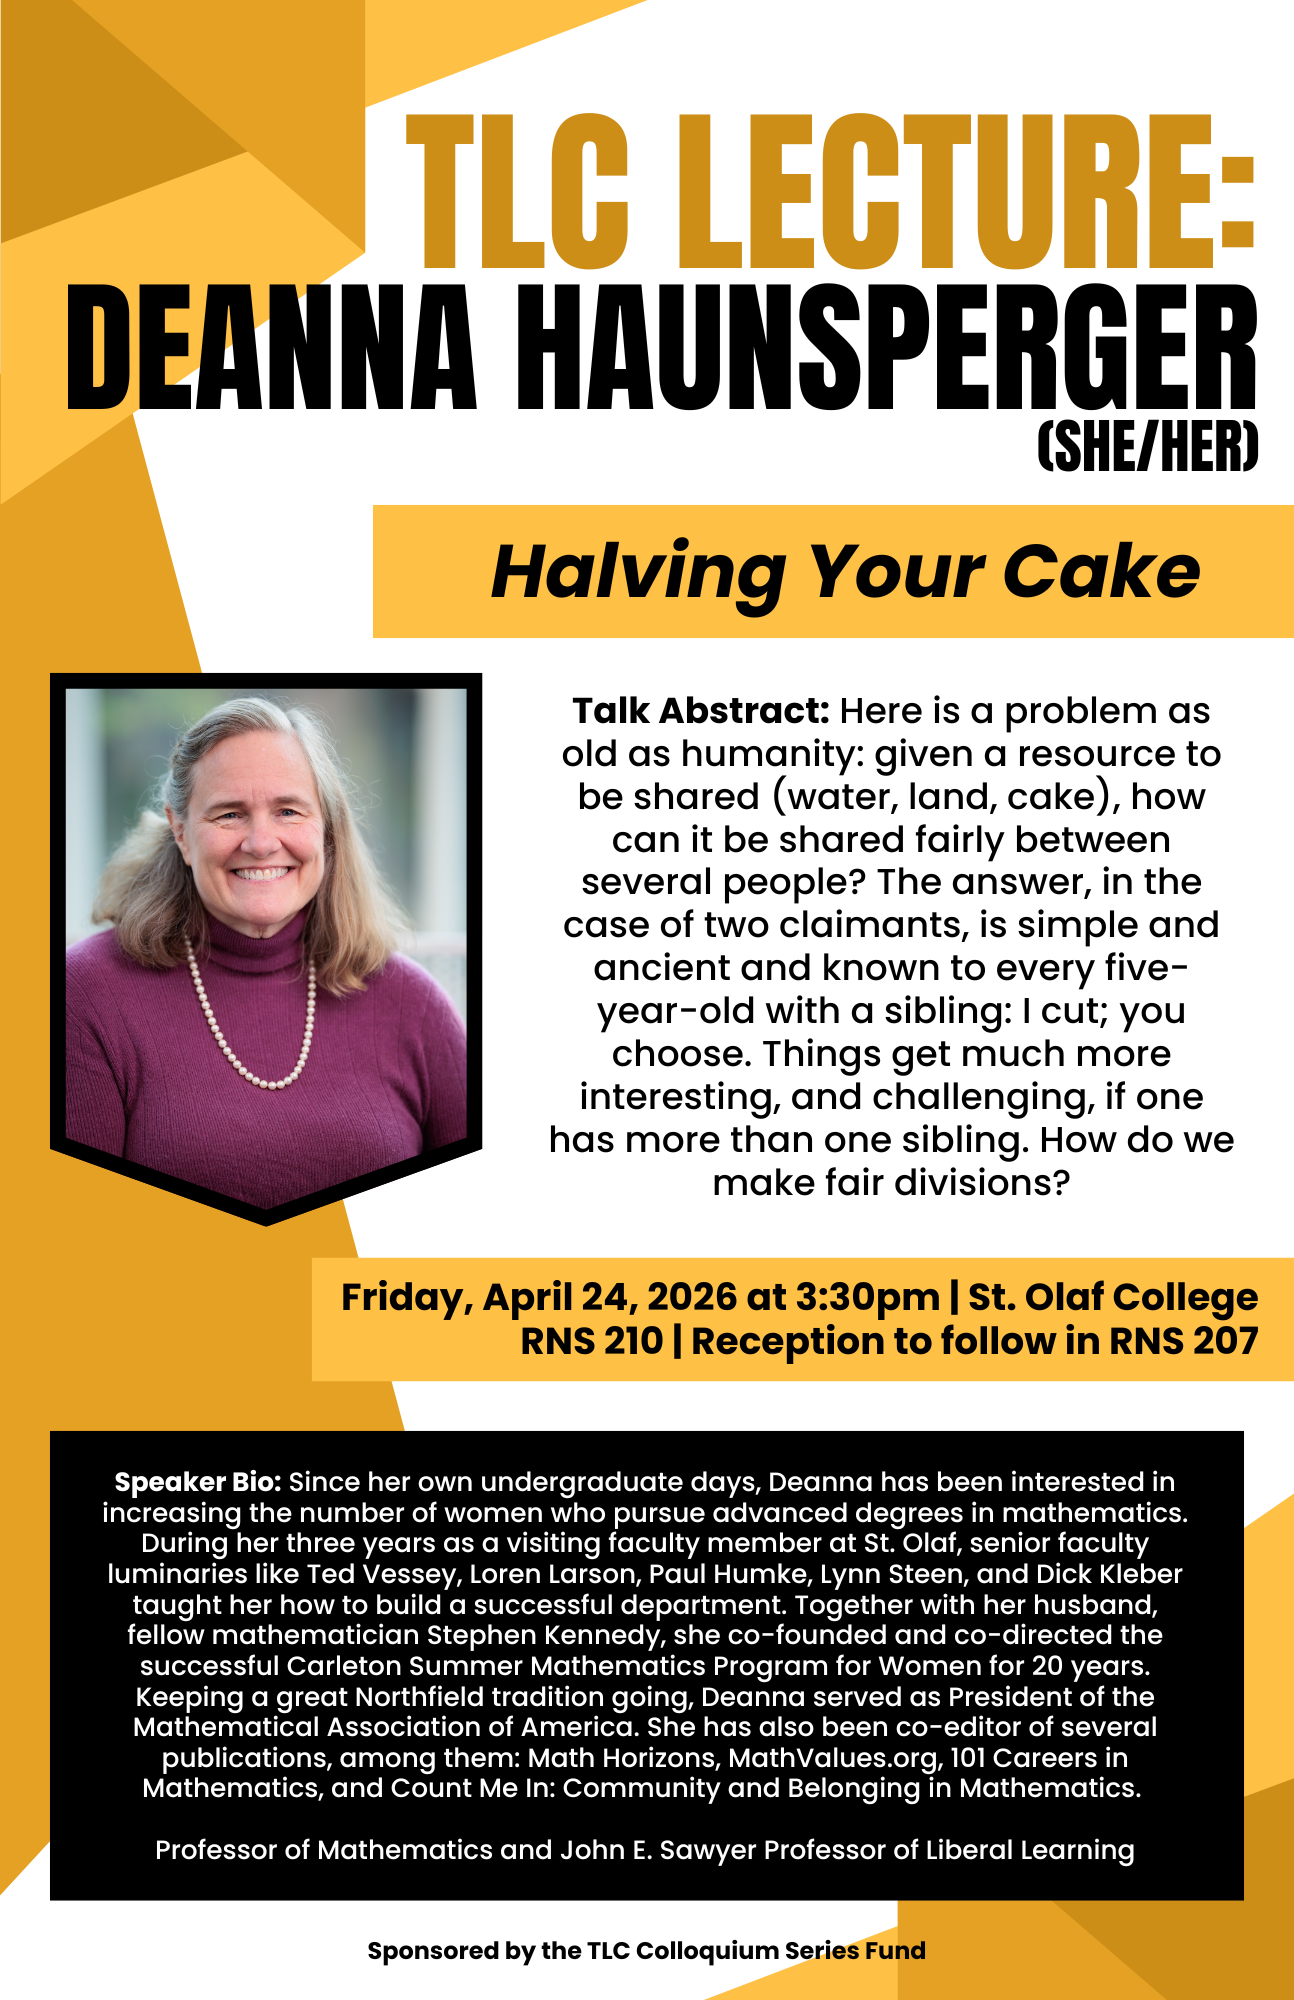
\includegraphics[height=0.95\textheight]{images/TLC Lecture Deanna Haunsperger.png}
\end{center}

\begin{center}
    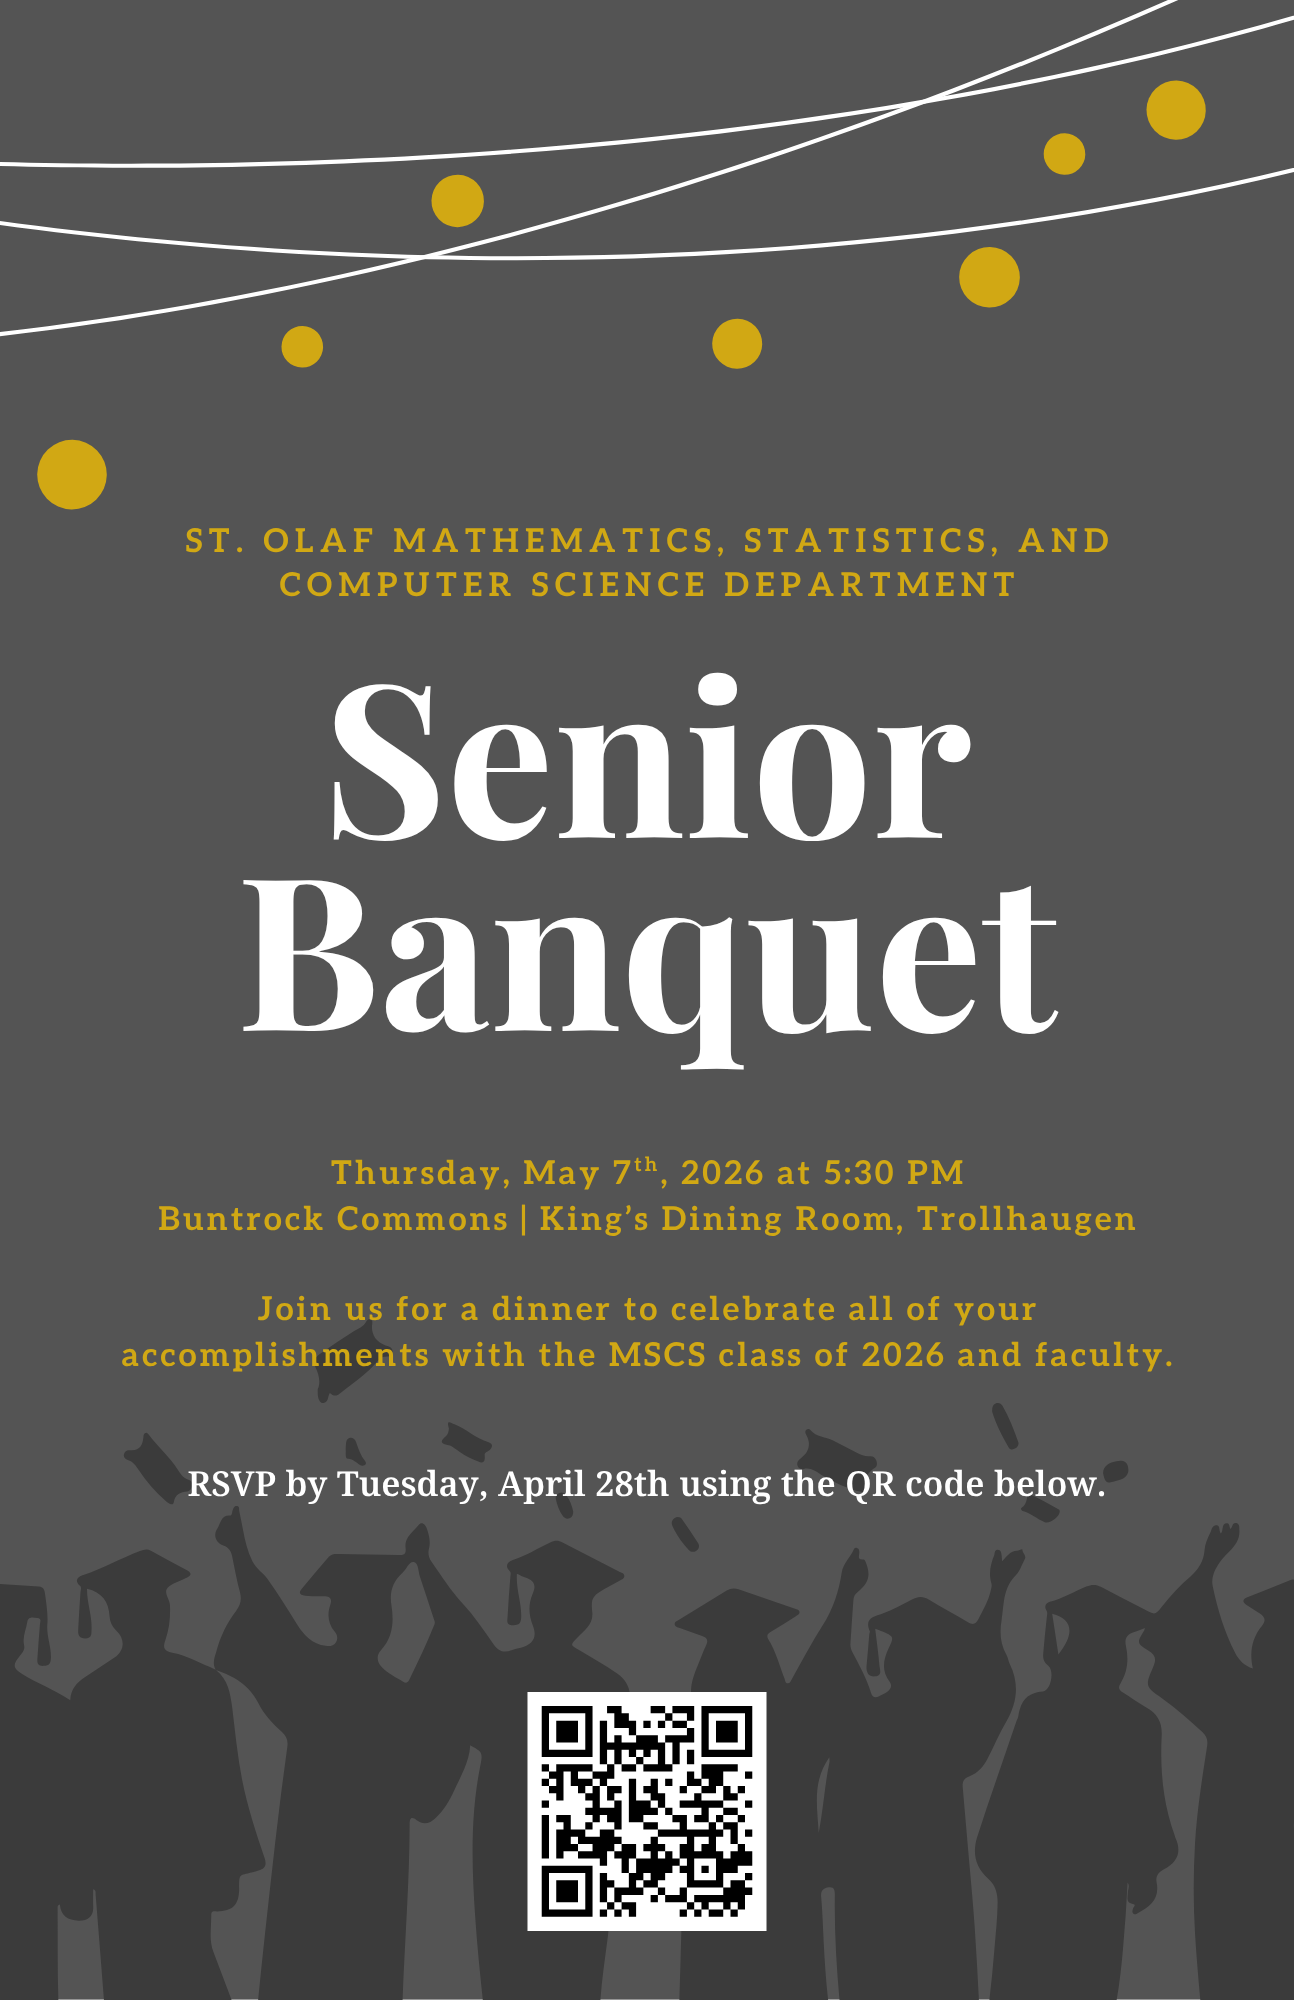
\includegraphics[height=0.95\textheight]{Senior Banquet 2026.png}
\end{center}

\begin{center}
    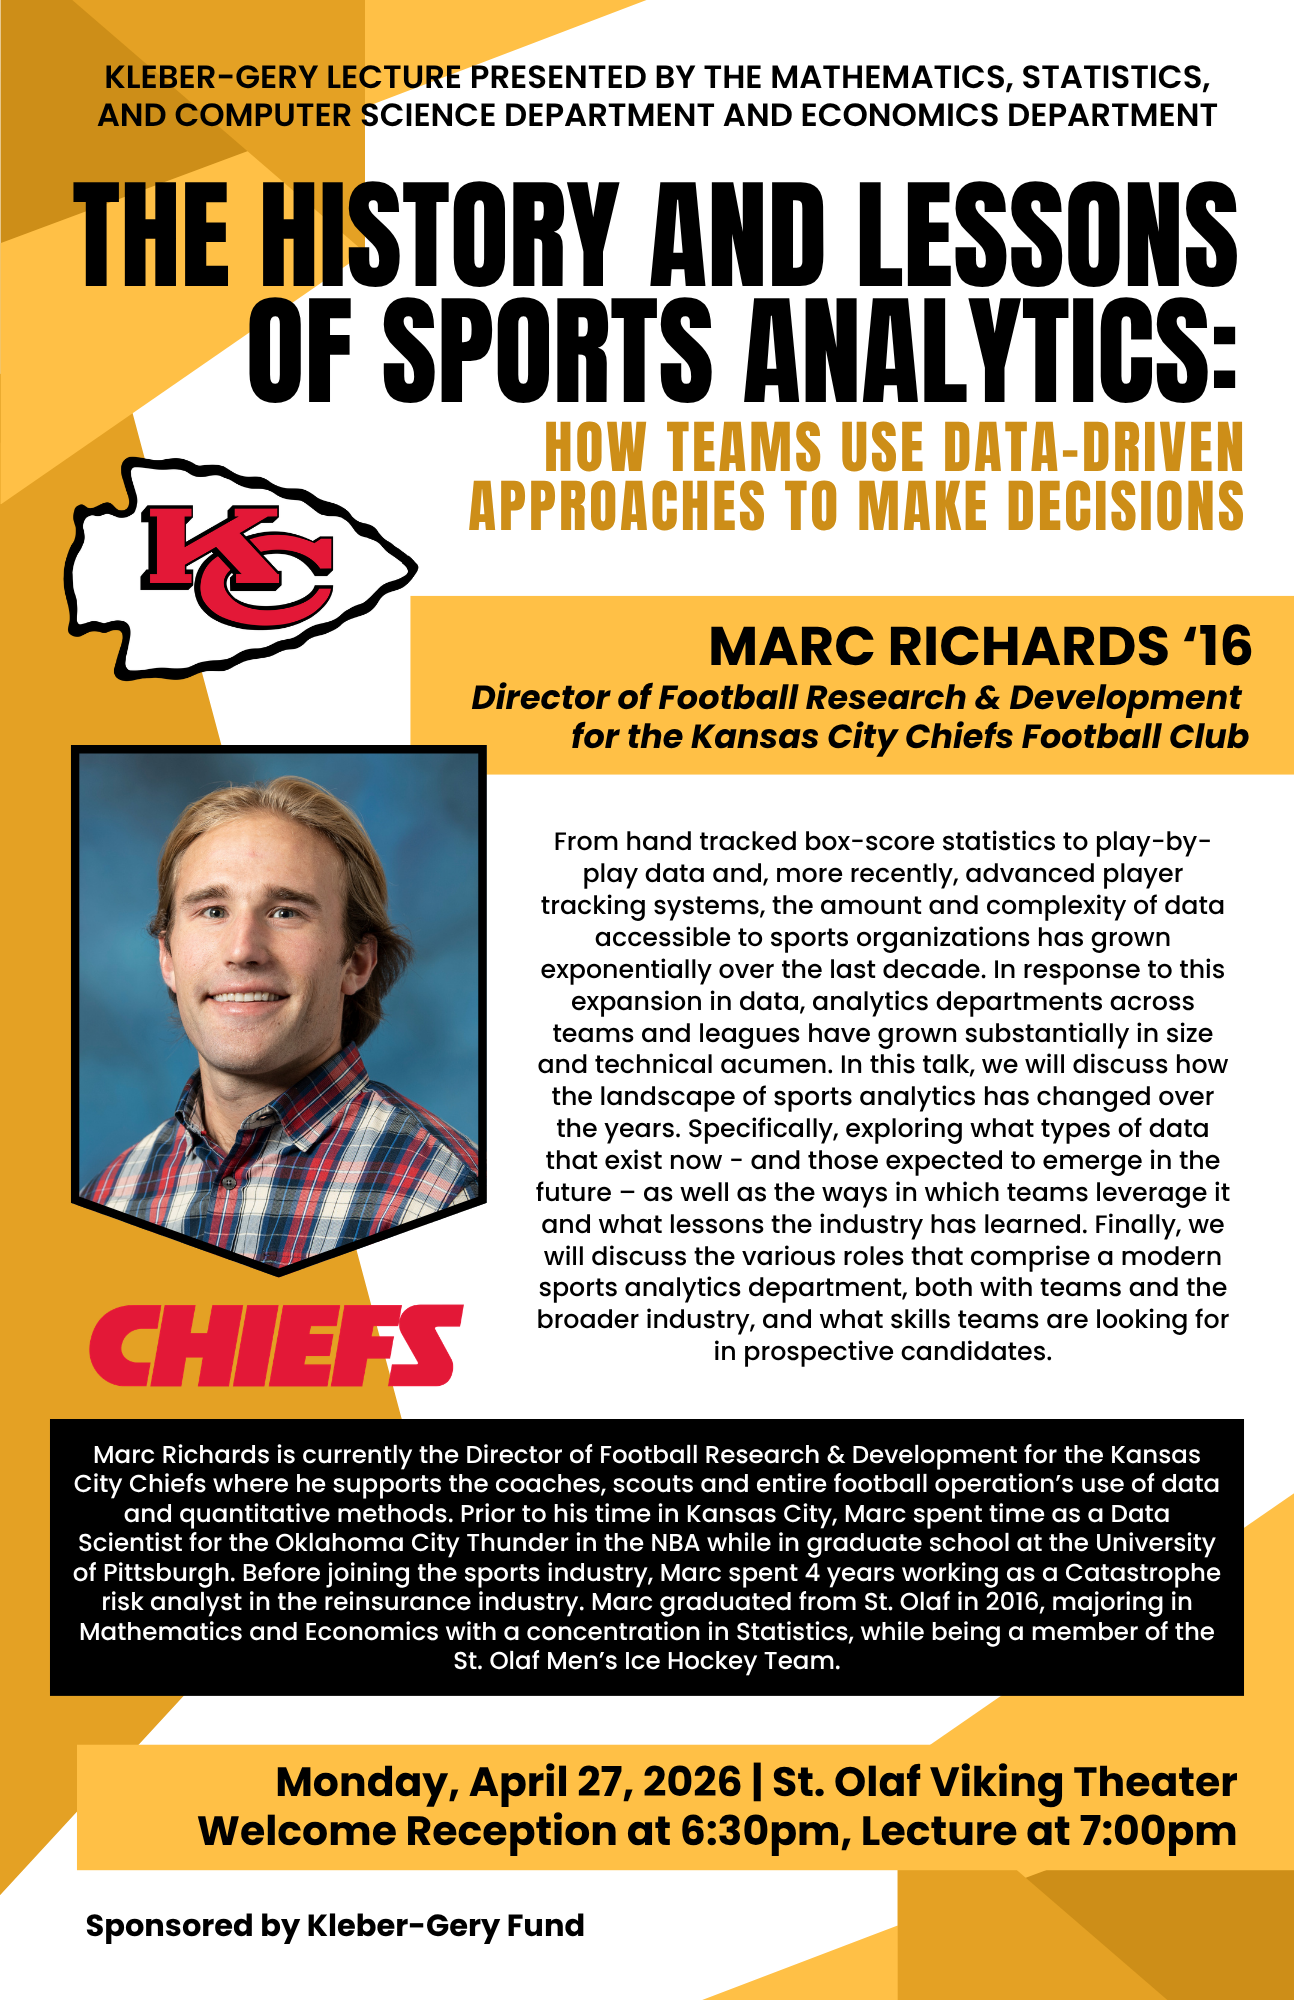
\includegraphics[height=0.95\textheight]{Kleber-Gery Evening Lecture with Marc Richards (2).png}
\end{center}

\begin{center}
    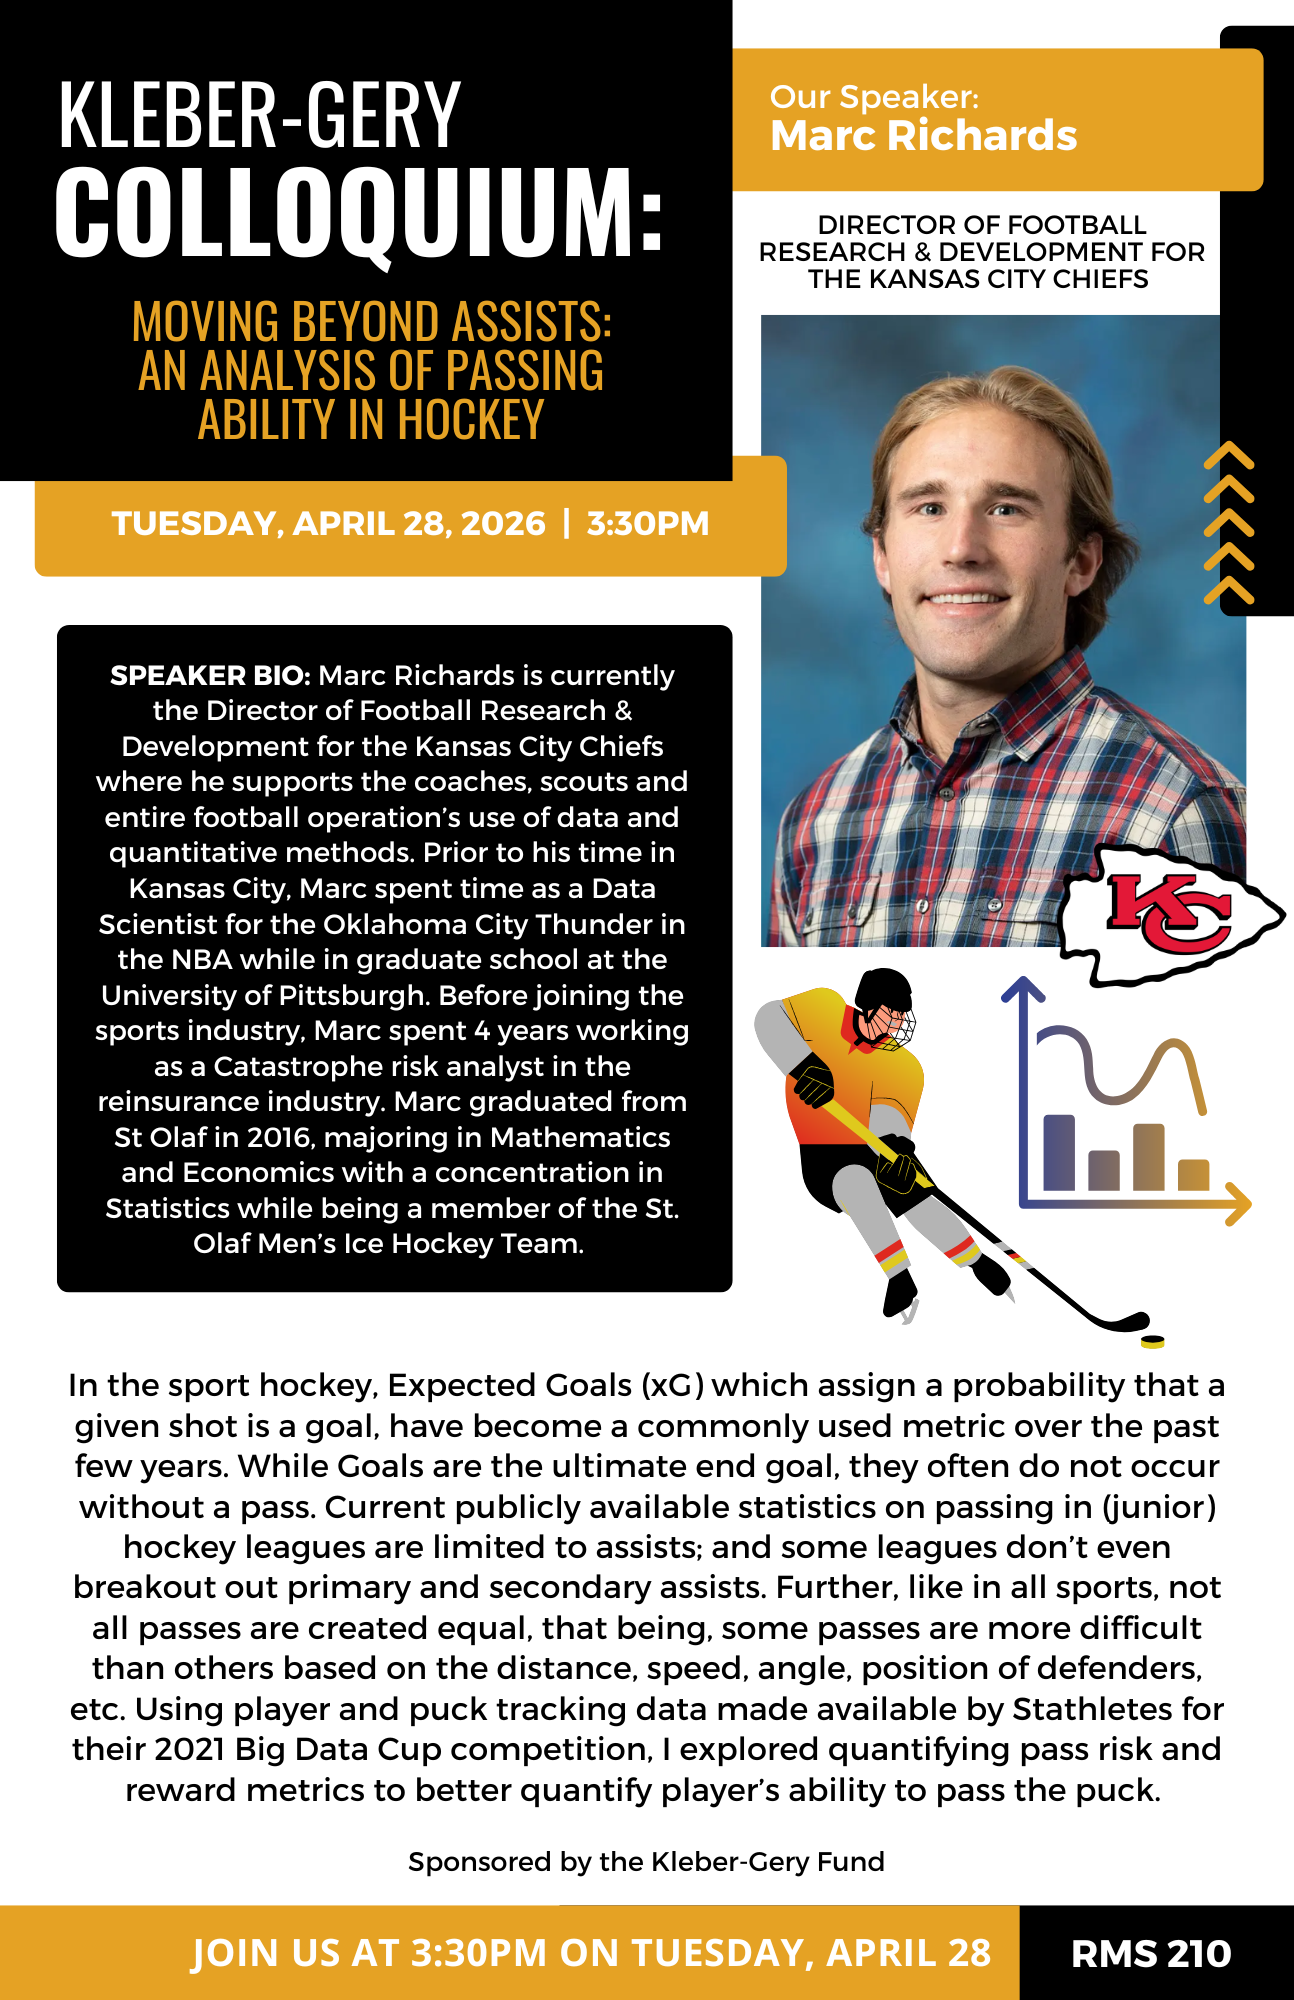
\includegraphics[height=0.95\textheight]{Kleber-Gery Colloquium Marc Richards (1).png}
\end{center}


\begin{center}
    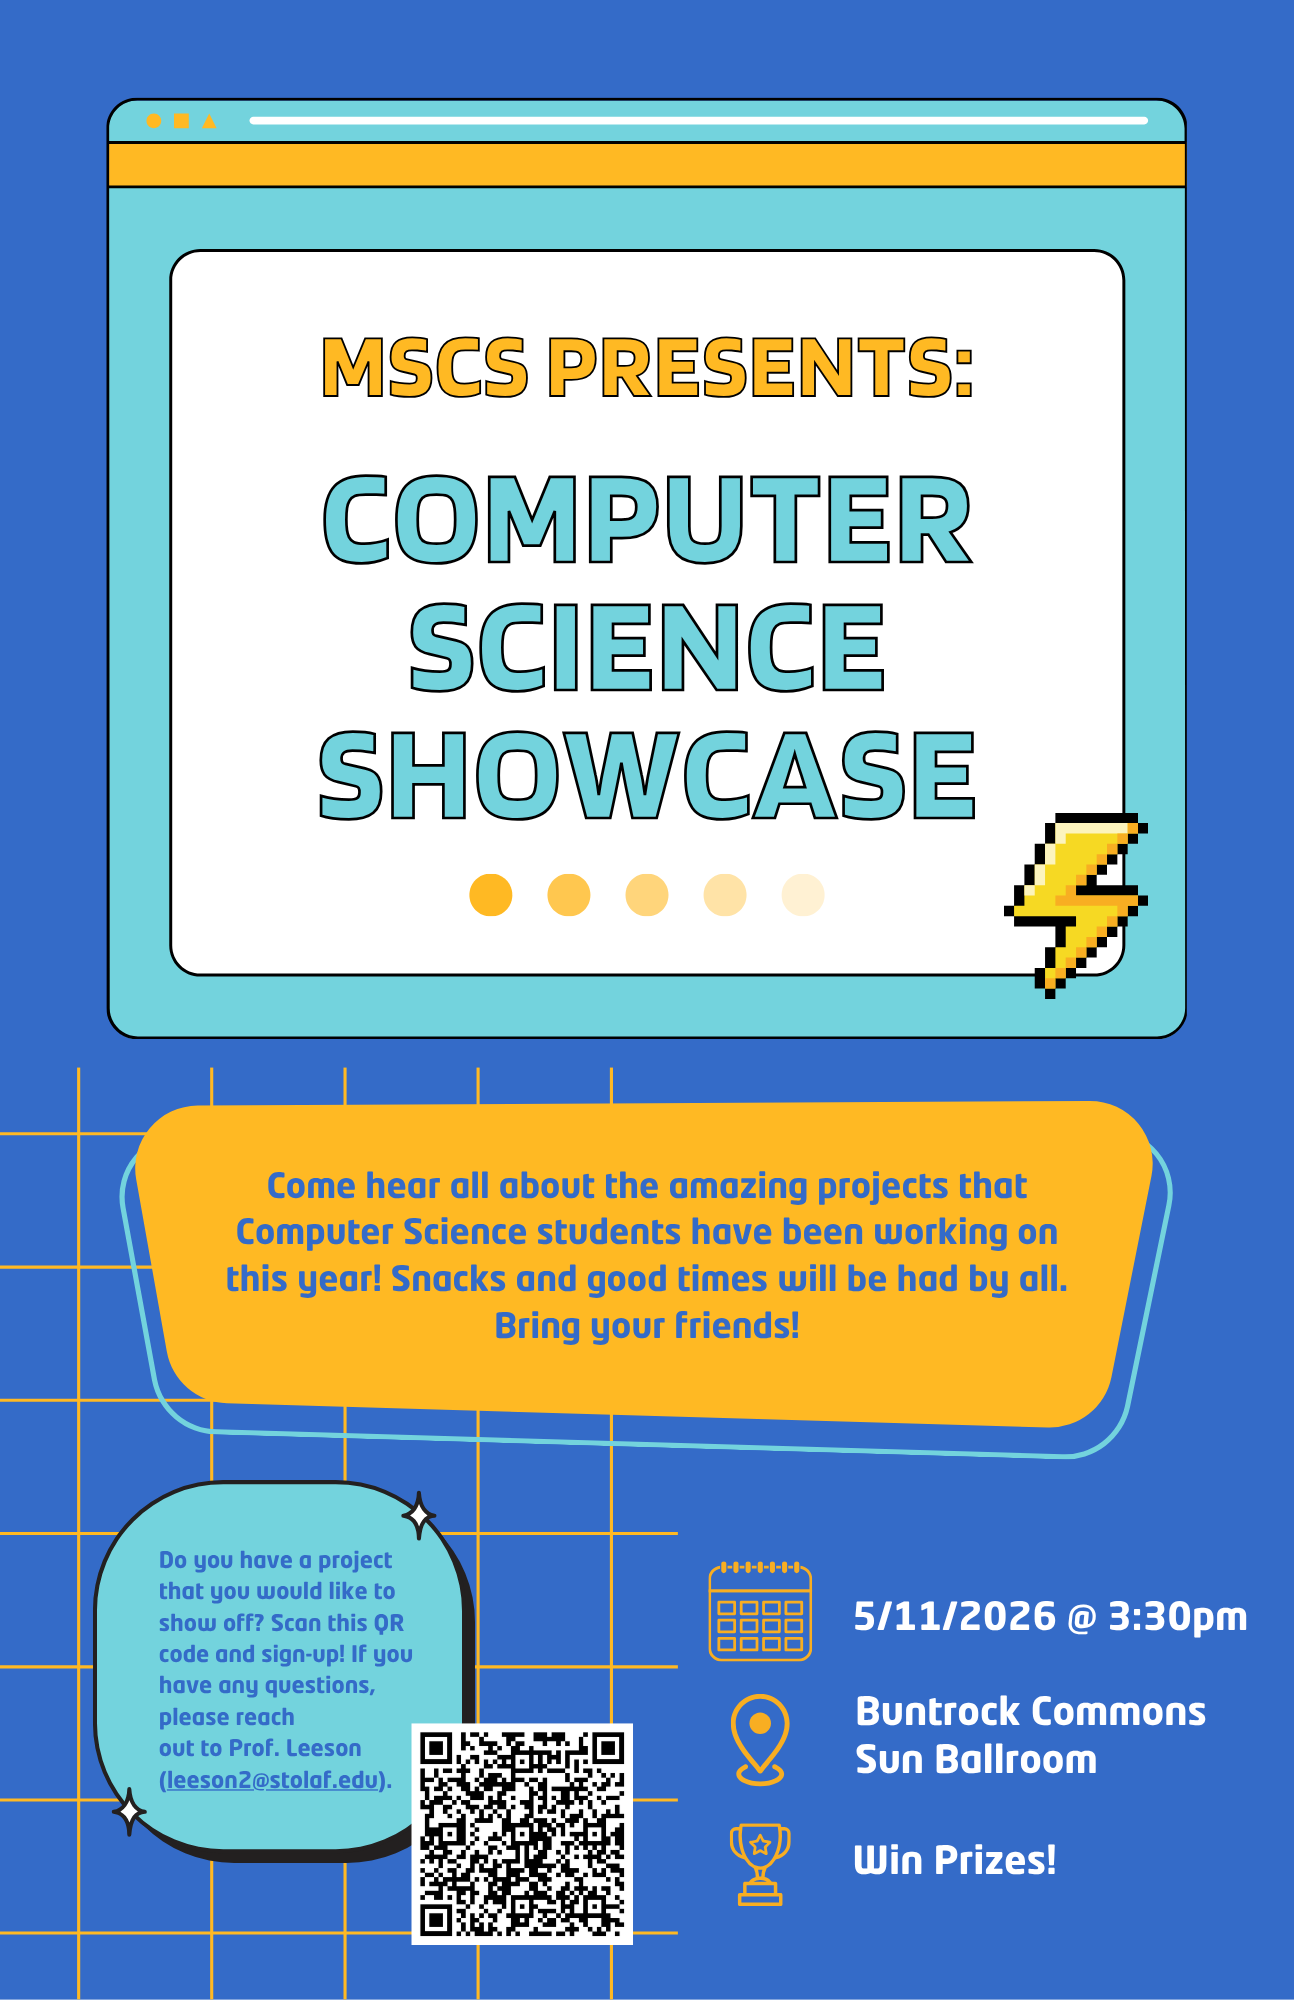
\includegraphics[height=0.95\textheight]{images/Computer Science Showcase (1).png}
\end{center}


\begin{center}
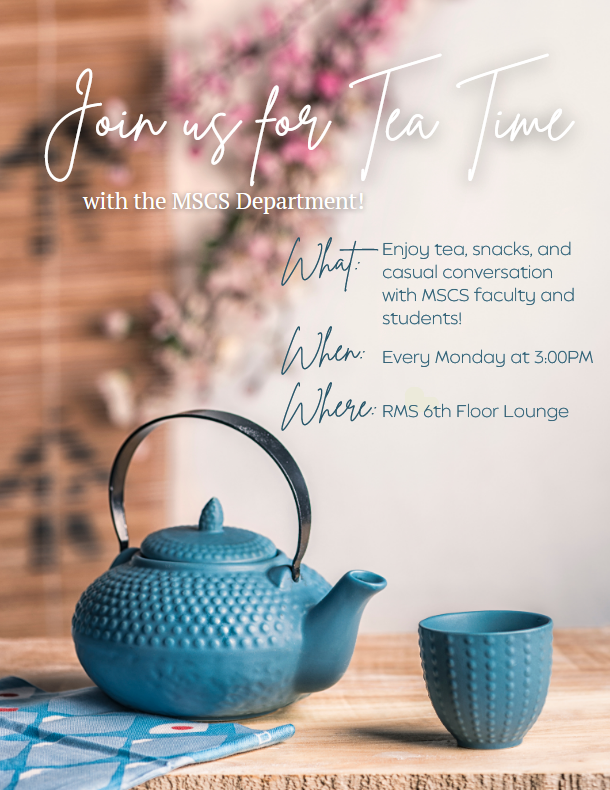
\includegraphics[width=0.9\textwidth]{images/Tea Time Poster.png}
\end{center}

\noindent{To submit an article, event, or anything else for publication in the Mess, email messeditor@stolaf.edu. Visit \href{https://wp.stolaf.edu/mscs/mscs-mess/}{http://wp.stolaf.edu/mscs/mscs-mess/} for a digital archive of previous MSCS Mess issues.}\\
	
\hfill Nima Dahir, Editor
	
\hfill Kyle Salois, Faculty Advisor


 

\end{document}